% 3456789012345678901234567890123456789012345678901234567890123456789012
%        1         2         3         4         5         6         7
%
% Format: LaTeX
%
% For information about this file, contact the author by email at
% joe.loughry@stx.ox.ac.uk, or by telephone: +44 (0)7984147430 (mobile), or
% +1 303 221 4380 (office).  The time zone is GMT minus 7 hours.
%

\documentclass{llncs}

% \usepackage[authoryear,sort&compress]{natbib}
% \usepackage[english,british]{babel}
% \bibliographystyle{alpha}

\bibliographystyle{splncs}

\usepackage{graphicx}

%
% end of preamble
%

\begin{document}
\title{Information Asymmetry in Classified Cross Domain System Accreditation}
\titlerunning{Information Asymmetry in Cross Domain}
\author{Joe Loughry}
\institute{Department of Computer Science, University of Oxford}

\maketitle

\begin{abstract}
The difficulty of cross domain systems security accreditation lies
inherent in the fact that, by definition, such systems always span at least
one boundary between security domains controlled by different data
owners. Consequently, approved solutions regularly encounter security
testing criteria that represent the duplicated responsibility for
residual risk of multiple security accreditors.  Each data owner perceives a
site-specific set of risks that would be desirable to mitigate,
a technology-dependent set of risks that it is possible to mitigate,
and a residual risk it is
felt acceptable not to mitigate.  Time and cost inefficiency in cross
domain system accreditation are shown to originate from asymmetry
of knowledge; Spence's criteria for market signalling are
shown to hold by analogy for accreditor--accreditor communication in the
presence of unequal or non-hierarchical security clearances.
By formalising signals, an efficient route to agreement about the true
level of residual risk might avoid repeated re-testing and redundant
risk mitigations.  If successful, the unnecessarily high cost of duplicated
security test and evaluation effort could be greatly reduced.
\end{abstract}

% \category{J.4}{Social and Behavioral Sciences}{Economics}
% \category{C.2.0}{Computer-Communication Networks}{General}[Security
% and protection (e.g., firewalls)]
% \category{D.2.4}{Software Engineering}{Software/Program Verification}[Validation]
% \category{J.7}{Computers in Other Systems}{Military}
% \terms{Economics, Validation}
% \keywords{Asymmetric knowledge, high assurance, certification and
% accreditation, cross-domain systems}

\section{Introduction}

`Sometimes it is necessary to violate your own security policy' \cite{Loughry2012b}.
A concrete example is the existence of cross domain systems,
whose reason for existence is to violate security policy in a controlled
manner~\cite{DCID-6/3a}.
Cross domain systems are interesting because they nearly always guarantee an adversarial
environment during validation testing.  Owners of classified
systems rarely trust outsiders---among whom
they number their users, their own software developers, owners of other
classified systems, and vendors or installers of cross domain solutions.

Caught in the crossfire of all this mistrust is the Designated Accrediting
Authority (DAA), a government official whose unenviable task it is to try to
determine the true level of risk in a system, reduce it to acceptable
levels, and then formally accept personal responsibility for the correct
operation of the system, on penalty of going to jail for a long time
if the cross domain system should fail in use.

In this paper we show that the DAA's predicament is the same thing as the
problem of market failure in the presence of asymmetric information familiar
to economic theory.  Furthermore the criteria for \emph{signalling}
established by Spence and Akerlof are met~\cite{Akerlof1970,Spence1973}.
This suggests a possible solution
to the present high cost of certification and accreditation of cross domain systems
that currently manifests in repeated testing and retesting of the same security criteria
by DAAs at different security classifications.

\subsection{Applicability}

This is an important problem for a specific, if not very visible, application area.
More generally, though, it is 
a microcosm of the problem of setting security parameters consistently
across a network of security devices in the cloud---but all occurring in one box.

\subsection{Organisation of the Paper}

The first part of this paper defines cross domain solutions and systems, designated
accrediting authority, and the assurance requirements of security
certification and accreditation for systems and networks handling
classified information.  Next, a simple example is used to motivate
the development of a model of DAA--DAA interaction that is sufficiently
powerful to reason about problems that have been observed to occur in
real situations.  The concept of residual risk is defined and
shown to be the primary driver of DAA decisions.  Cross domain system accreditations
have a tendency to prompt ineffectual
repeated testing because of security clearance rules that limit inter-DAA
communication; this leads to high
costs.  Economic theories of asymmetric knowledge are shown to be
applicable to the problem.  Finally, a solution is proposed using an
artificial market to resolve the asymmetry and reach an improved
equilibrium resulting in lower overall cost.

\subsection{Purpose of this Paper}

The purpose of this paper
is to put forth the idea and validate whether or not working accreditors
are likely to find the proposed tool useful.

\section{Cross Domain Systems and Cross Domain Solutions}

Cross domain solutions are needed anywhere that security boundaries exist.
`In our real-world environment made up of multiple single-level networks---that is,
relatively isolated networks each of which comprises a security enclave or
domain at a particular security classification---connectected to the
network cloud, it is often necessary to move information across security
boundaries, and by the Intermediate Value Theorem for Computer Security (CS-IVT),
at least one multi-level component must exist in the
cloud'~\cite[\textsection 6.2]{Bell2005b,Loughry2012b}.  A cross domain solution or
\emph{controlled interface} is employed to interconnect systems or networks
in different security domains, thereby forming a Cross Domain System,
or CDS~\cite{DCID-6/3a}.
By definition, CDS installations always span at least one boundary between
security domains controlled by different data owners~\cite{Loughry2010a}.

In the most general case, data owners nearly always mistrust one another,
because the relationship between their security classifications may be
non-hierarchical, or incommensurable, or simply equipotent, as happens in
international
installations~\cite{TSOL_2.5_CMW}.  Cross domain solution developers and installers regularly
encounter situations that have no clear precedent yet need to be resolved;
they do this by means of a combination of high-assurance
software/hardware and through negotiation with data owners and security accreditors.

Each data owner is represented by a designated accrediting authority
whose job it is to approve connection of the cross domain solution to
a classified system or network and to permit operation for a specified period of
time~\cite{NIST-SP-800-37,NIST-SP-800-53A2,DIACAP,NIST-SP800-53r3}.
DAAs work closely with the cross domain solution developer or installer and other DAAs to ensure
adequate protection of the classified information in their security domain.
Data owners worry about two potential threats: accidental compromise of the confidentiality of
classified information outside the security boundary (called a spill),
and negative impacts to the integrity or availability of their information
from the introduction of malicious code or denial-of-service attacks.  DAAs,
being people, 
in addition operate under the constraints of their government security clearance and
security classification rules.

\section{A Model of DAA Interactions Constrained by Different Security Clearances}

Figure~\ref{figure:simplest-possible-CDS} shows a very simple example of
a CDS that is nevertheless sufficient to illustrate the problem.
There is generally no DAA for unclassified systems, so let us say that the
low side is classified Confidential and the high side is at a higher classification.
The low-side DAA---by convention, cross domain solution developers habitually
refer to data flows as being `low to high' or `high to low' despite the
fact that the distinction may be a matter of opinion depending on the data
owner's
perspective---represents the United States Department of Defence because the information
on the low side is at a collateral classification, that is, it is classified but not
protected by additional code words.  But because the high side contains Sensitive
Compartment Information (SCI), which has a non-hierarchical relationship to
collateral security classifications, the high-side DAA must represent one of the members of the
Intelligence Community (IC), for example the National Geospatial-Intelligence
Agency (NGA).
Real cross domain systems commonly are more complicated, with multiple data flows in more than one
direction, more than two endpoints, conditional information flows dependent on content,
sanitisation, transliteration, and non-hierarchical security classification relationships.

In our model, DAAs having responsibility for information at different
classification levels have security clearances and accesses that match
their responsibilities.  In the real world, that might not be true; all
DAAs might be cleared for Top Secret/SCI.  Our model presupposes the more
limited case for two reasons: firstly, because it better reflects the
intent of security policy irrespective of administrative convenience, and
secondly because it allows us to analyse the important case of international
CDS installations, where DAAs most definitely do not share mutual clearances.

\begin{figure}[htbp]
    % 'trim' specifies how much to remove from left, bottom,
    % right, and top edges of an A4 size PDF page.
    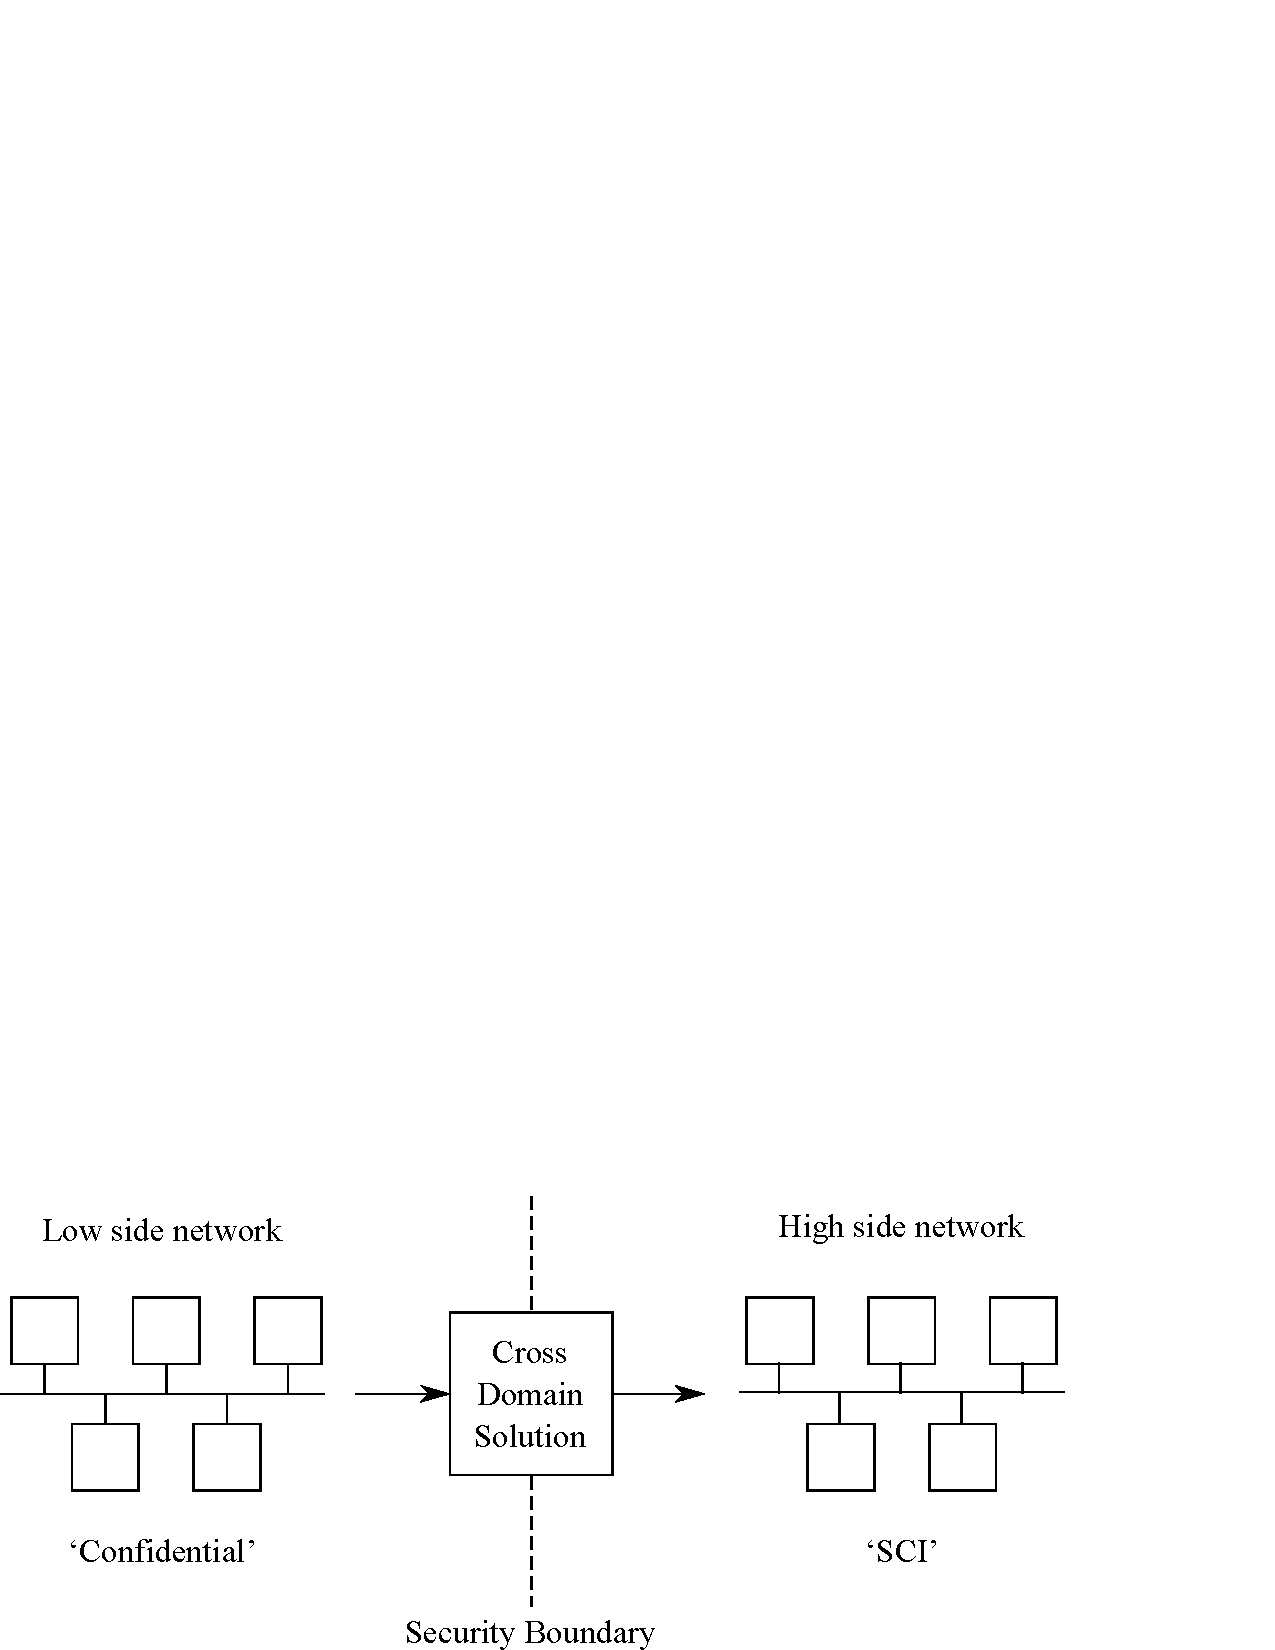
\includegraphics[width=\textwidth,trim=0 19cm 2cm 0,clip]{simplest-possible-CDS.pdf}
    \caption{A simple cross-domain system with asymmetric information.  The low security side
		is classified CONFIDENTIAL and the high side is Sensitive Compartmented Information (SCI).}
    \label{figure:simplest-possible-CDS}
\end{figure}

Consider the following situation.  DAA~1 holds a Confidential security
clearance and has need-to-know, so is therefore privy to classified
information about certain threats that are known to exist by the data
owner of the low-side system.  DAA~1 perceives a site-specific set of
risks $A_1$ that affect the low side system, each risk computed from the \emph{probability} of
occurrence of an identified \emph{threat} leading to an \emph{impact} which is derived
from the value of the asset~\cite{Flechais2005}.
Risks can be avoided, mitigated, transferred, or accepted~\cite{Tockey2004}.
DAA~1 assesses
a set of risks based on the known threats at his or her clearance, the
best available estimate of the probability of
occurrence $pT_i$ of each, and the value $V$ of the information on the low side as
perceived by the low side data owner; this
set of risks that DAA~1 thinks it would be desirable to mitigate is:
\begin{equation}
A_1 = \bigcup_i[pT_i\times V]
\end{equation}
where $0 \leq pT_i < 1$.

DAA~2 holds a Top Secret/SCI security clearance with accesses similarly determined
by DAA~2's need-to-know.  It can be understood that DAA~2 knows about
some highly classified
threats that are not known to DAA~1.  In practice, DAA~2 should be aware
of all the threats that DAA~1 knows about, but this is not required by
the model.  DAA~2 perceives a site-specific set of risks $A_2$ affecting
the high side based on probably a larger set of known threats, an estimate
$pT_j$
of their probability of occurrence, and the value $V^\prime$ of the information on the
high side as perceived by the high side data owner.  This is the set of
risks that DAA~2 thinks would be desirable to mitigate:
\begin{equation}
A_2 = \bigcup_j[pT_j\times V^\prime]
\end{equation} where $0 \leq pT_j < 1$.

$A_2$ is not necessarily a proper superset of $A_1$ or even needs be
larger than $A_1$.
DAA~1 values low side information independently of DAA~2, and quite
possibly assesses different probabilities for similar risks---although if
they are seriously different, it might be better to treat them as distinct
threats---simply because it is DAA~1's own asset on the line.  Similarly, DAA~2
values high side information independently of DAA~1.

DAA~1 perceives a technology-dependent set of risks $B_1$ that it is
possible to mitigate, and DAA~2 similarly perceives a set of risks $B_2$
that is is possible to mitigate.
Because both sides are presumed to be aware of what is technically
possible, it is likely that $B_1 = B_2$, although there is always the
possibility that DAA~2 is aware of some highly classified risk mitigation
for a threat that DAA~1 does not even know exists.

\section{The Idea of Residual Risk}

The job of a DAA
is formally to accept responsibility on behalf of the Principal Accrediting
Authority (PAA) for the \emph{residual risk} of connecting their classified information system
to the overall CDS.  Residual risk for each DAA $i$ is defined as the relative complement
$A_i-B_i$, being the set of risks which it is felt, by that DAA, to be acceptable
not to mitigate.  The goal of the DAA is always to minimise residual risk.

This is
achieved through a combination of choosing the right cross domain solution vendor and product
based on Certification Test and Evaluation (CT\&E) results, correctly configuring
the cross domain solution according
to its technical capabilities, and rigorous testing of the CDS before and
after issuance of Approval-to-Connect (ATC) to verify that the CDS adequately protects
the security domain of the data owner each DAA represents.  In real installations,
the PAA responsible for the highest-classification information in the CDS generally is
responsible for choosing a cross domain solution vendor.  The process of testing a
cross domain solution in situ forming a CDS
is called Security Test and Evaluation (ST\&E) and results,
in our model, in the granting of an Approval
to Operate (ATO) from each DAA.  ATO lasts for a limited amount
of time, usually three years, and is periodically reviewed.

\section{Asymmetric Knowledge}

To reiterate, by definition a CDS installation always
spans at least two security domains controlled by different data owners.
With multiple data owners come multiple DAAs.  With each DAA, under present rules, comes
another round of ST\&E, oftentimes performed by the same team of Independent
Verification and Validation (IV\&V) contractors for reasons
described in~\cite{Loughry2010a}.

It is from the asymmetry of knowledge
just described that the well-known time and cost inefficiency of the CDS
accreditation process arises.
If the true level of residual risk could be agreed upon by all DAAs and
validated by a single round of ST\&E to the satisfaction of all parties,
then the cost of CDS accreditation would be greatly reduced.  Towards that goal,
we now show that the problem is isomorphic to a well-known result from economic
theory.

Problems that can be caused by asymmetry of information are well
understood.
In markets characterised by a lack of knowledge on the part of
buyers, rational behaviour by all participants can lead to a collapse
of the market to the point where no seller will offer a product for
sale~\cite{Akerlof1970}.
Conversely, in markets characterised by a lack of knowledge on the
part of sellers, \emph{adverse selection} results in a lopsided distribution
of risk, which can lead to a situation called \emph{moral hazard} in which
participants who know they are insulated from the consequences of a
risk behave differently than if they were fully exposed to it~\cite{Crosby1905}.
Game theory offers a handful of compensating strategies for asymmetric
knowledge, among them the concept
of \emph{signalling}~\cite{Spence1973,Stigler1961}.  In signalling,
sellers in a market under conditions of asymmetric information
can resolve the asymmetry by communicating information to buyers in a
convincing way, but in order for the buyer to believe the signal, the cost
of asserting the signal must be high~\cite{Spence1973}.

Can we apply these ideas to the problem of improving the situation of a
temporary non-optimal equilibrium amongst the individual assessments
of $n$ different DAAs about the total residual risk resulting from the
installation of a complex CDS?  In one sense, the problem is that
non-communicating DAAs can end up stuck in isolated local minima
because they lack an important piece of information
about a risk mitigation
already implemented by another DAA in response to a threat the existence
of which is above the first DAA's clearance level.\footnote{The related problem
of highly classified
threats for which there is no known risk mitigation is a very real one,
but in the absence of a fix, from the perspective of a higher-cleared
DAA it is a worry he or she cannot talk about, and from the perspective of a
lower-cleared DAA, ignorance is bliss.}  In another sense, the problem
is analogous to a covert channel, through which we wish to communicate
some information in violation of the system security policy~\cite{NCSC-TG-030}.
In that case, the security policy we need to violate is not that of the CDS, but of
the security clearances of some of the DAAs.

Is it even meaningful to talk about a single value for the residual risk
of a complex CDS interconnecting many different security enclaves, thereby
exposing data of widely differing perceived---and maybe even objectively
intrinsic---values to the risk of damage, disclosure, or loss?  It is
attractive to call the overall residual risk
\begin{equation}
R = \sum_i (A_i - B_i)
\end{equation}
from the residual risks assessed by each DAA---who is, after all,
responsible
for the safety of data in his or her security enclave---because this metric behaves
the right way in the intuitive sense that if one DAA feels that the residual
risk to one enclave is unusually high, it properly increases the overall
level of risk of the CDS.

\section{Proposed Solution}

With that out of the way, let us consider the problems of simulating a
market amongst DAAs who are constrained (in the most general case) from
communicating freely about their individual assessments of residual risk
of a CDS because of security classification rules.
It is a weird sort of market in which participants offer to buy and
sell commodities that they do not know the value of, although someone else
does.  Since some of the DAAs are prohibited from describing the exact details
of a threat or a risk mitigation, or in some important cases the lack of
any known risk mitigation for a threat with no countermeasure, they must
in some way signal (in Spence's use of the word) the actual value of the
residual risk as they perceive it.  The traditional view of signals holds
that for the signal to be convincing, it must have a high cost to preclude
dishonest use of signals to gain unfair advantage.  We believe that the cost
constraint is satisfied in this adaptation of the model because there
is negative incentive for cheating when the result of dishonesty---that is,
to communicate
a false high reading of the residual risk as perceived by DAA~$k$---would
either raise the value of $R$, increasing the amount of risk that
DAA~$k$ must accept formal responsibility for, or conversely, artificially
depress the apparent level of risk below what DAA~$k$ knows the true
value to be, again raising the level of personal risk to DAA~$k$'s own self
when he or she signs on the dotted line.

\subsection{The Criteria for Signalling Are Met}

The required high cost of signals in this market is made
manifest by the very real risk that a cleared DAA takes in choosing to
communicate information about the true level of residual risk in violation
of his or her oath to protect classified information.  It works both
ways, as even DAAs with low security clearance understand the need-to-know
rule and would hesitate to casually provide classified information to another
absent a clearly communicated need-to-know decision from their authorised
security officer.  The necessary and sufficient criteria for signalling, therefore, are
met~\cite[pp.\ 499--500 and 367, respectively]{Akerlof1970,Spence1973}.

\subsection{Turf Wars}

One final aspect remains to be examined.  This is the seldom-acknowledged
incidence of `turf wars' in the DAA community.  We have
observed in CT\&E activities, and have anecdotal reports from
practising DAAs in ST\&E, of prima facie obstructionist behaviour exhibited
by accreditors and their supporting casts of penetration testers
against cross domain solution developers and in some cases even against other DAAs.
The reasons for such activity are not yet clear.  The outcome, however,
leads almost always in the direction of increased accreditation cost; in
the worst case, pathological turf wars could even lead to another well known
economics result, the tragedy of the commons~\cite{Hardin1968}.

\section{Summary and Future Work}

The main contribution of this paper is that we have shown
that the market for residual risk satisfies Spence's criteria for signalling
in~\cite{Spence1973}.  We have not yet constructed or tested a simulation
of the DAA market for information, but intend to do that in future work
after receiving feedback from the accreditation community about the
applicability of the model in this paper.

A new tool being developed at the University of Oxford, called {\it nihil obstat},
is designed to facilitate the determination of an equilibrium in the market for
residual risk amongst DAAs by soliciting a series of bid/ask quotations from
accreditors at different security classification levels and using them to set a
`market price' for the residual risk that each DAA is prepared to accept.

% Accreditors might exchange information or not.  If they exchange
% information, nothing more can be said.  If they do not, it could
% be because they do not have any information to exchange.  Or it
% could be that they have information, and would like to exchange it
% but are prohibited by security clearance or security classification
% rules.  Or they might not want to exchange information.  One reason
% for that could be turf wars.  Turf wars have been observed in
% practice.  Reasons for turf wars include\ldots

\section*{Acknowledgements}

The author wishes to thank his supervisors, including Andrew Martin, who observed
that the author seemed to be trying to build a covert channel machine, and Ivan
Fl\'echais, who gave the clearest formulation of risk yet.

This paper is dedicated to the memory of Sister Rosemary Fiori, S.L.

\bibliography{consolidated_bibtex_file}

\end{document}

